\section{Kecerdasan Buatan}
\subsection{Definisi Kecerdasan Buatan}
 \hspace{1cm} Artificial Intelligence (AI) atau Kecerdasan Buatan adalah simulasi kecerdasan manusia, yang dimodelkan dalam mesin dan diprogram untuk berpikir seperti manusia. Dengan kata lain, kecerdasan buatan adalah sistem komputer yang dapat melakukan tugas-tugas yang biasanya membutuhkan manusia atau kecerdasan.
 
\hspace{1cm} McLeod & Schell, 2007. Artificial Intelligence (AI) adalah aktivitas yang memberikan mesin seperti komputer kemampuan untuk menampilkan perilaku yang dianggap cerdas, seolah-olah kemampuan tersebut ditampilkan oleh manusia.

\subsection{Sejarah dan perkembangan Kecerdasan Buatan}
\hspace{1cm}Sejauh ini, John McCarthy telah memberikan kontribusi besar dalam sejarah pengembangan AI. McCarthy (McCarthy) menciptakan bahasa pemrograman tingkat tinggi yang disebut LISP, yang digunakan oleh sebagian besar kecerdasan buatan saat ini. Belakangan, McCarthy membuat program, yang disebutnya program dengan akal sehat. Dalam program tersebut, McCarthy merancang sebuah teknologi yang dapat menyelesaikan masalah tersebut. Pada tahun 1959, Nathaniel Rochester dan beberapa murid IBM-nya membuat program AI yang disebut Geometry Theorm Prover. Program ini dapat digunakan untuk membuat teorema menggunakan pernyataan yang ada.


\hspace{1cm} Namun, sekitar tahun 1960-an dan 1970-an, perkembangan kecerdasan buatan melambat. Ini karena kecerdasan buatan yang muncul saat ini hampir tidak tahu apa-apa tentang produknya. Keberhasilan penggunaan produk kecerdasan buatan hanyalah hasil dari operasi sederhana. AI mulai berkembang kembali dan menjadi industri pada tahun 1980. Berawal dari Digital Equipment Corporation (DEC), perusahaan menemukan sistem bernama R1 yang dapat digunakan untuk mengkonfigurasi sistem pada komputer baru. Pada tahun 1988, R1 telah menjalankan 40 sistem dan berhasil menghemat biaya operasi perusahaan hingga 40 juta dollar setiap tahun. Di tahun yang sama, hampir semua perusahaan besar di Amerika Serikat memiliki departemen sendiri untuk mengembangkan AI. Akibatnya, pendapatan tahunan sebagian besar perusahaan di Amerika Serikat telah meningkat menjadi 2 miliar dollar per tahun.

\hspace{1cm}Di Indonesia belum ada ilmuwan yang berhasil menciptakan teknologi kecerdasan buatan yang diakui dunia. Namun, banyak anak muda seperti Digital Nativ telah mengembangkan dan terus menggunakan teknologi ini untuk berinovasi. Bahkan Digital Nativ, teknologi yang mereka kembangkan, memadukan unsur artistik dan alam.


\subsection{Supervised learning, Unsupervised Learning, Klasifikasi, Regresi}
\begin{enumerate}
     \item Supervised learning adalah jenis pembelajaran terbimbing yang mengetahui keluaran yang diharapkan sebelumnya. Biasanya pembelajaran ini dilakukan dengan menggunakan data yang ada. Dalam metode ini, setiap mode yang disediakan ke jaringan saraf tiruan memiliki keluaran yang diketahui. Mode masukan akan ditetapkan ke neuron di lapisan masukan. Pola tersebut akan menyebar di sepanjang jaringan saraf ke neuron di lapisan keluaran. Lapisan keluaran akan menghasilkan pola keluaran, yang kemudian akan cocok dengan pola keluaran target. Sekarang, jika ada perbedaan antara mode keluaran hasil pembelajaran dan mode keluaran target, akan terjadi kesalahan. Jika nilai kesalahan ini masih cukup besar berarti perlu pembelajaran lebih lanjut.
     
     \item Unservised Learning adalah algoritme pembelajaran mesin yang digunakan untuk menarik kesimpulan dari kumpulan data. Metode ini hanya akan mempelajari data berdasarkan kedekatannya atau biasa disebut clustering. Metode pembelajaran tanpa pengawasan yang paling umum adalah analisis cluster, yang digunakan dalam analisis data untuk menemukan pola atau pengelompokan tersembunyi dalam data. Dalam algoritme pembelajaran tanpa pengawasan, data tidak memiliki label yang jelas, dan model dapat belajar dari data dengan mencari pola implisit. Sangat berbeda dengan supervised learning, unsupervised learning merupakan pembelajaran yang hanya memiliki variabel input tetapi tidak ada variabel output yang berhubungan. Tujuan dari pembelajaran mesin adalah untuk memodelkan struktur data dan mendapatkan fungsi untuk mendeskripsikan data.

    \item Klasifikasi adalah salah satu topik utama dalam penambangan data atau pembelajaran mesin. Klasifikasi adalah pengelompokan data dimana data yang digunakan memiliki label atau kategori sasaran. Oleh karena itu, algoritma yang digunakan untuk menyelesaikan masalah klasifikasi dapat dibagi menjadi supervised learning atau supervised learning. Tujuan dari supervised learning adalah membuat label atau data target berperan sebagai "supervisor" atau "guru", yang mengawasi proses pembelajaran untuk mencapai tingkat akurasi atau presisi tertentu.
    
    \item Regresi adalah metode statistik yang digunakan di bidang keuangan, investasi dan disiplin ilmu lainnya. Kuncinya adalah menentukan kekuatan dan karakteristik hubungan antara variabel dependen (biasanya diwakili oleh Y) dan serangkaian variabel lain (disebut variabel independen).
 \end{enumerate}

\subsection{Data Set, Training Test, Testing Test}
\begin{enumerate}
    \item Data set dalam data mining, data masukan data yang akan diolah disebut juga data set. Kumpulan data merupakan kumpulan dari objek data atau biasa disebut catatan, titik, vektor, pola, kejadian, pengamatan, kasus atau bahkan data. Ada banyak cara untuk merepresentasikan suatu kumpulan data, misalnya atribut yang digunakan untuk mendeskripsikan tipe objek (yang dapat bersifat kualitatif atau kuantitatif). Atribut ini adalah faktor atau parameter yang menyebabkan terjadinya kelas / tag / objek. Contoh dataset ini adalah data bias yang didapat dari media sosial, Twitter, Instagram atau data publik lainnya.
    
    \item Training Set Training set adalah bagian dari kumpulan data yang kami latih untuk membuat prediksi atau menjalankan fungsi algoritme ML. Kami memberikan petunjuk melalui algoritme sehingga mesin yang kami latih dapat menemukan korelasi atau mempelajari pola dari data yang diberikan.

    \item Testing set digunakan untuk mengukur klasifikasi pengklasifikasi yang benar. Oleh karena itu, data dalam set pengujian tidak boleh berada dalam set pelatihan sehingga Anda dapat melihat apakah model pengklasifikasi "pintar" dalam klasifikasi.
\end{enumerate}


\section{Instalasi}
\begin{enumerate}
    \item Instalasi library scikit dari anaconda dengan pip install -U scikit-learn
     \begin{center}
    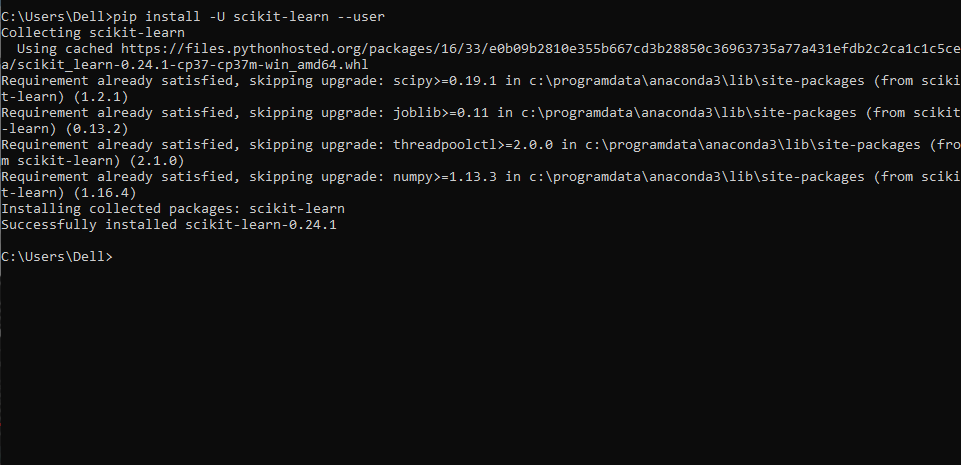
\includegraphics[width=.8\textwidth]{figures/1184098/chapter 1/00.png}
    \end{center}
    \item Mencoba Loading an example dataset, dengan membuka link yang sudah tertera pada Main dan mengambil salah satu example dan jalankan spyder dan lihat hasilnya
     \begin{center}
    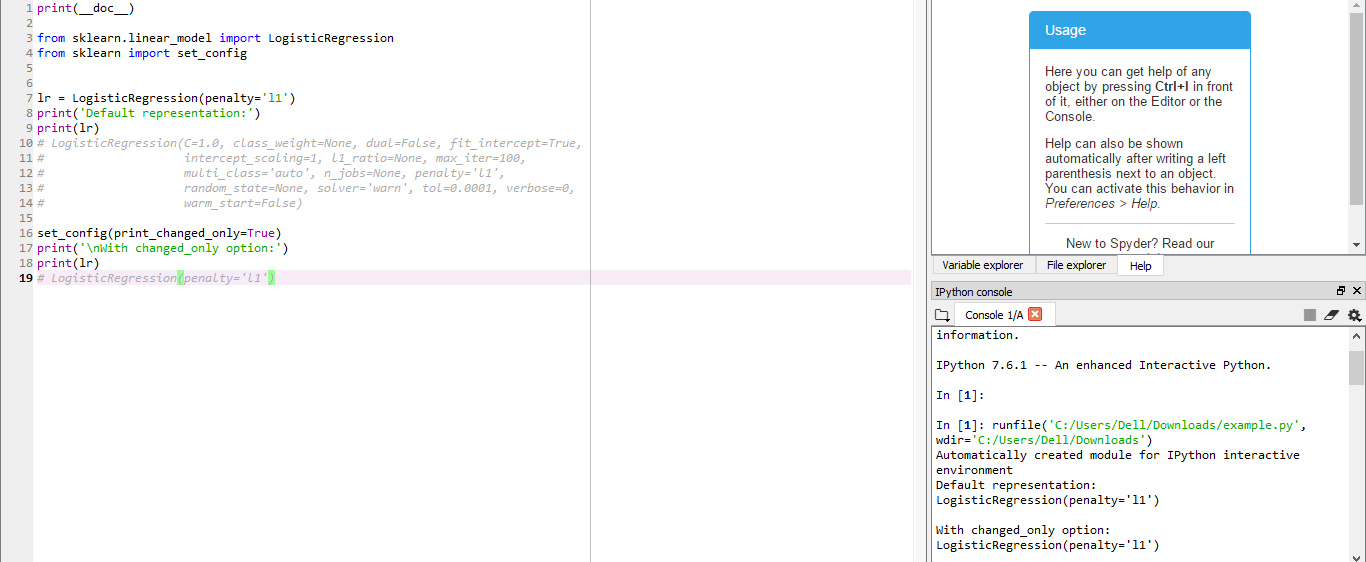
\includegraphics[width=.8\textwidth]{figures/1184098/chapter 1/01.png}
    \end{center}
    \item Mencoba Learning and predicting, dengan membuka link sebelumnya dan mencari learning dan predicting, lalu buat file baru pada spyder dan run
    \begin{center}
    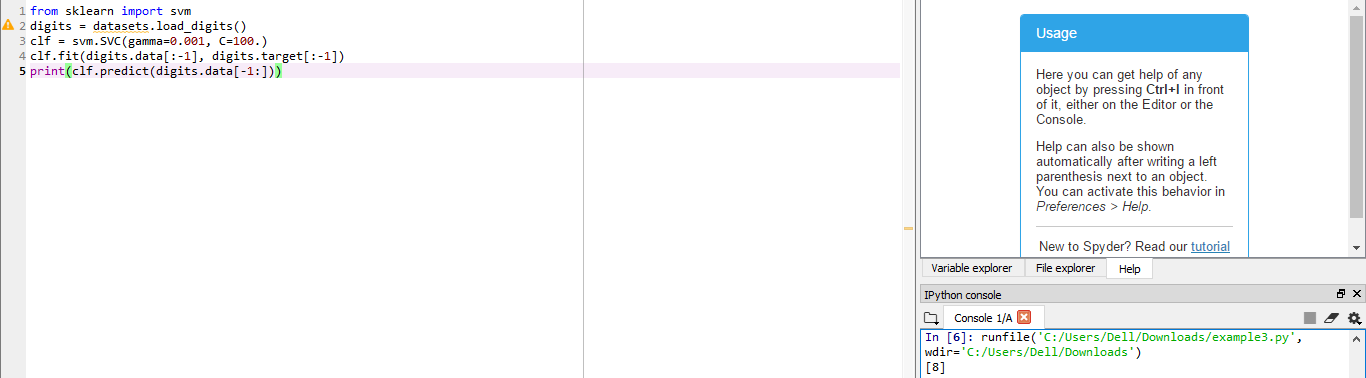
\includegraphics[width=.8\textwidth]{figures/1184098/chapter 1/03.png}
    \end{center}
    \item mencoba Model persistence, dengan membuka link sebelumnya dan mencari persistence, lalu buat file baru pada spyder dan run
    \begin{center}
    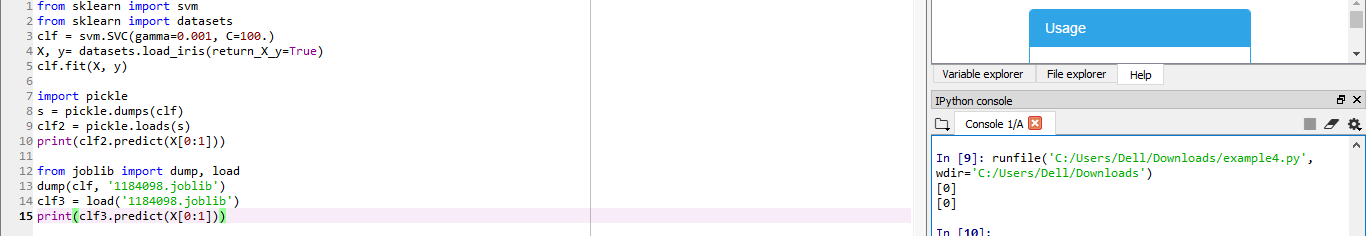
\includegraphics[width=.8\textwidth]{figures/1184098/chapter 1/04.png}
    \end{center}
    \item Mencoba Conventions, dengan membuka link sebelumnya dan mencari convestion, lalu buat file baru pada spyder dan run
     \begin{center}
    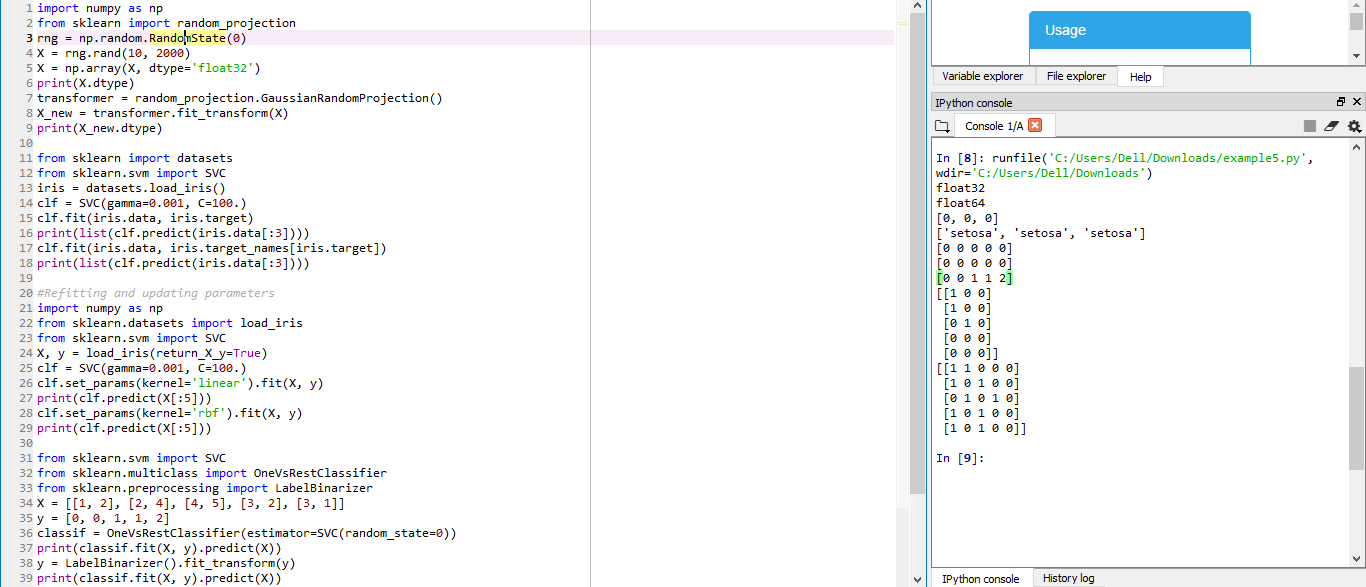
\includegraphics[width=.8\textwidth]{figures/1184098/chapter 1/05.png}
    \end{center}
\end{enumerate}

\section{Error dan Penanganannya}
\begin{enumerate}
    \item Ditemukan error pada file example3.py yaitu ModuleNotFoundError: No module named 'sklear'
      \begin{center}
    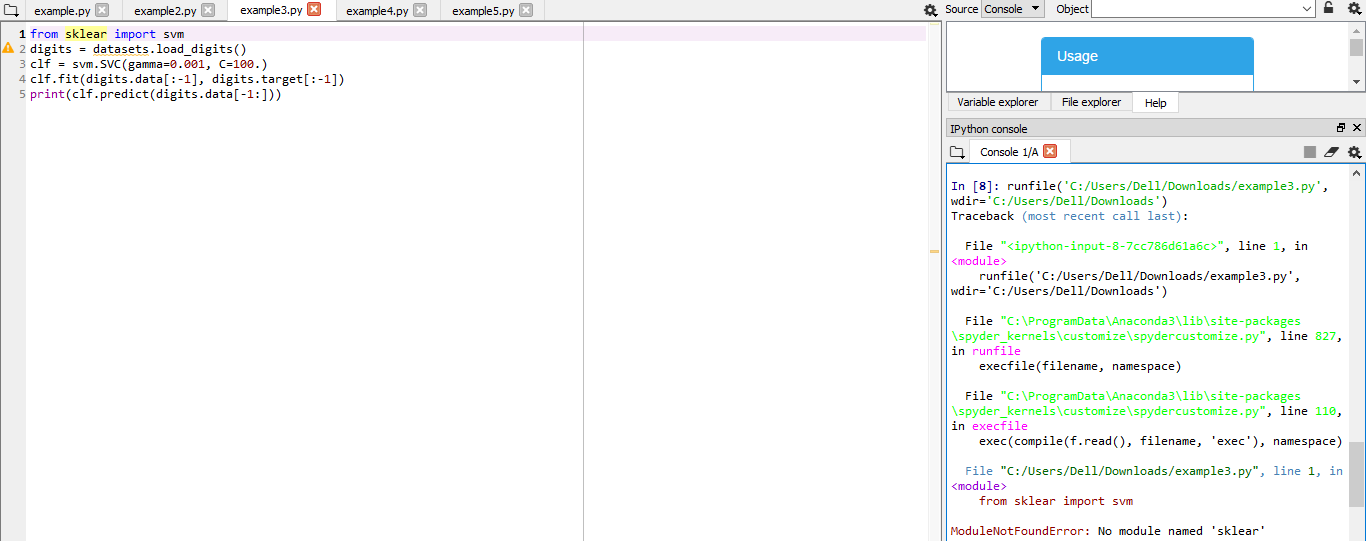
\includegraphics[width=.8\textwidth]{figures/1184098/chapter 1/erro1.png}
    \end{center}
    \item kode eror dan jenis errornya
    \item Untuk penangananya yaitu seharusnya penulisan library nya harus teliti sehingga saat mengimport class dataset pada library scikit learn dapat berjalan dan tidak error. 
     \begin{center}
    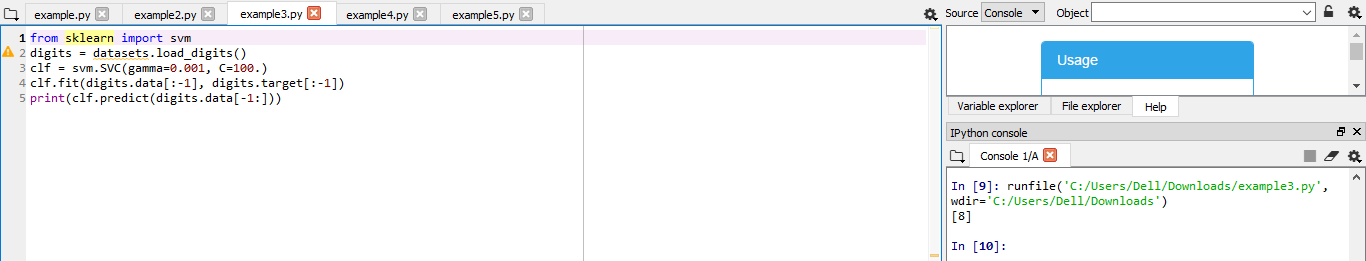
\includegraphics[width=.8\textwidth]{figures/1184098/chapter 1/error2.png}
    \end{center}
\end{enumerate}


